\documentclass[sigconf]{acmart}

\usepackage{graphicx}
\usepackage{hyperref}
\usepackage{todonotes}

\usepackage{endfloat}
\renewcommand{\efloatseparator}{\mbox{}} % no new page between figures

\usepackage{booktabs} % For formal tables

\settopmatter{printacmref=false} % Removes citation information below abstract
\renewcommand\footnotetextcopyrightpermission[1]{} % removes footnote with conference information in first column
\pagestyle{plain} % removes running headers

\newcommand{\TODO}[1]{\todo[inline]{#1}}

\begin{document}
\title{Using Machine Learning Classification of Opioid Addiction
for Big Data Health Analytics}

  \author{Sean M. Shiverick}
  \affiliation{%
  \institution{Indiana University Bloomington}
}
\email{smshiver@indiana.edu}

\renewcommand{\shortauthors}{S.M. Shiverick}

%%%%%%%%%%%%%%%%%%%%%%%%%%%%%%%%%%%%%%%%%%%%%%%%%%%%%%%%%%%%%%%%%%%%%%%%%%%%%%%%

\begin{abstract}
Classification of opioid addiction can identify important features relevant 
for predicting drug abuse and overdose death. Machine learning procedures were 
applied to data from a large National Survey of Drug Use and Health (NSDUH-2015) 
to classify individuals for illicit opioid use according to demographic 
characteristics and mental health attributes (e.g., depression). Classification 
models of opioid addiction can be extended for big data health analytics to 
include high-dimensional datasets, data collected over previous years, or 
expanded to the larger population of patients taking prescription opioid 
medication. The results seek to raise awareness of risk factors related to 
opioid addiction among patients and medication prescribers, and help 
decrease the risk of opioid overdose death. 
\end{abstract}

\keywords{Health Analytics, Machine Learning Classifiers, Opioid Addiction, 
Big Data, i523, hid335}

\maketitle

%%%%%%%%%%%%%%%%%%%%%%%%%%%%%%%%%%%%%%%%%%%%%%%%%%%%%%%%%%%%%%%%%%%%%%%%%%%%%%%%
\section{Introduction}

Big Data offers tremendous potential to fuel innovation and transform society. 
Can this momentum be harnessed to address a serious health crisis such as the 
opioid overdose epidemic? \cite{cdc16} Health informatics is generating huge 
amounts of data at a rapid pace, from electronic medical records (EMRs), 
clinical research data, to population-level public health data \cite{herland14}. 
This project considers health analytics from two levels, the research questions 
being addressed and the data used to answer them. The question of interest in 
this project is whether opioid dependency and addiction can be predicted from 
demographic attributes and psychological characteristics. Survey research 
provides data on a wide range of issues that people may be reluctant to 
disclose, including mental health disorders, personal medical health concerns, 
prescription medications, and illicit drug use. Responses to surveys may be 
biased to some degree, but measures of confidentiality and anonymity help to 
assure more accurate disclosures. The goal of this project is to use machine 
learning procedures to classify individuals susceptible to opioid abuse and 
dependence. Understanding the features that contribute to opioid addiction 
can identify underlying risk factors and increase awareness of potential 
opioid abuse for patients and health care providers. The results could be 
extended to big data from previous years of the opioid crisis and to the 
larger population of patients taking prescription opioid mediation. Different 
machine learning classification methods are discussed.


%%%%%%%%%%%%%%%%%%%%%%%%%%%%%%%%%%%%%%%%%%%%%%%%%%%%%%%%%%%%%%%%%%%%%%%%%%%%%%%%
\subsection{Opioid Overdose Epidemic}

The abuse of prescription opioid medication in the U.S. has become a major 
health crisis of epidemic proportions \cite{volkow14}. Over 2 million Americans 
were dependent or abused prescription opioids such as oxycodone or hydrocodone 
in 2014\cite{cdc17}. Overdose deaths from prescription opioids have quadrupled 
since 1999, resulting in more than 180,000 deaths between 1999 to 2015 
\cite{nida17}. Drug overdose deaths increased significantly for males and 
females, between 25-44 years, ages 55 and older, for Non-Hispanic Whites and 
Blacks, in the Northeast, Midwest, and Southern regions of the U.S.
\cite{cdc16}. Mobile health applications can monitor patient medication 
consumption and provide an early warning system for potential abuse, detecting 
sudden changes in medications, higher dosages, or rapid escalation of a 
prescribed dosage \cite{varshney13}. Reliable information about medication 
dosages can be difficult to obtain based on self-reports. Individuals dependent 
or addicted to prescription opioids may obtain synthetic opioids such as 
fentanyl or illicit drugs such as heroin. Because the dosage levels and potency 
of illicit opioids are largely unknown, there is greater risk of drug overdose 
death. The sharp increase in overdose deaths due to synthetic opioids (other 
than methadone) has coincided with the increased availability of illicitly
manufactured fentanyl, which is indistinguishable from prescription fentanyl. 
The findings indicate the opioid overdose epidemic is getting worse, and 
requires urgent action to prevent opioid dependence, abuse and overdose death. 
The target group for this project is individuals who reported misusing or 
abusing prescribed opioid medication who also used heroin, shown in Figure 1. 

%%%%%%%%%%%%%%%%%%%%%%%%%%%%%%%%%%%%%%%%%%%%%%%%%%%%%%%%%%%%%%%%%%%%%%%%%%%%%%%%
\subsection{Machine Learning Approaches} 

Machine learning is a set of procedures and automated processes for extracting 
knowledge from data. The two main branches of machine learning are supervised 
learning and unsupervised learning. Supervised learning problems involve 
prediction about a specific target variable or outcome of interest. If a given 
dataset has no target outcome, unsupervised learning methods can be used to 
discover underlying structure in unlabeled data. The goal of this project is 
to classify opioid addiction and focuses on supervised learning. Supervised 
learning is used to predict a certain outcome from a given input, when examples 
of input/output pairs are available \cite{muller17}. A machine learning model 
is constructed from the training set of input-output pairs, to predict new test 
data not previously seen by the model. The two major approaches to supervised 
learning problems are regression and classification. When the target variable 
to be predicted is continuous, or there is continuity between the outcome 
(e.g., home values, or income), a regression model is used to test the set of 
features that predict the target variable. If the target is a class label, set 
of categorical or binary outcomes (e.g., `spam` or `ham`, `benign` or 
`malignant`), then classification is used to predict which class or category 
label that new instances will be assigned to.

%%%%%%%%%%%%%%%%%%%%%%%%%%%%%%%%%%%%%%%%%%%%%%%%%%%%%%%%%%%%%%%%%%%%%%%%%%%%%%%%
\subsection{Classification Algorithms} 

Comparing the performance of different learning algorithms can be helpful for 
selecting the best model for a given problem \cite{raschka17}. One of the 
simplest classification algorithms is K-Nearest-Neighbors (KNN) which takes 
a set of data points and classifies a new data point based on the distance 
(e.g., Euclidean, by default) to its nearest neighbors. The main parameter for
KNN is the number of neighbors, and k of 3 or 5 neighbors works well. The 
advantage of the KNN classifier is that it provides a solution that is easy to 
understand. A limitation of KNN is that it does not perform well with a large 
number of features (100 or more) or sparse datasets. Several different 
classification algorithms are considered below.

\subsubsection{Logistic Regression Classifier}

Logistic regression is a commonly used linear model for classification problems. 
The decision boundary for the logistic regression classifier is a linear function 
of the input; a binary classifier separates two classes using along a line, 
plane, or hyperplane. Linear classification models differ in terms of (1) how 
they measure how well a particular combination of coefficients and intercept fit 
the training data, and (2) the type of regularization used \cite{muller17}. The 
main parameter for linear classification models is the regularization parameter 
`C`. High values of C correspond to less regularization and the model will fit 
the training set as best as possible, stressing the importance of each individual 
data point to be classified correctly. By contrast, with low values of C, the 
model puts more emphasis on finding coefficient vectors (w) that are close to 
zero, trying to adjust to the `majority` of data points \cite{muller17}. In 
addition, the penalty parameter influences the coefficient values of the linear 
model. The L2 penalty (Ridge) uses all available features, but pushes the 
coefficient values toward zero. The L1 penalty (Lasso) sets the coefficient 
values for most features to zero, and uses only a subset for improved
interpretability. This paper uses a logistic regression classifier to predict 
Heroin use from demographic attributes, mental health, prescription opioids, medication use, misuse, and illicit drug use. 

%%%%%%%%%%%%%%%%%%%%%%%%%%%%%%%%%%%%%%%%%%%%%%%%%%%%%%%%%%%%%%%%%%%%%%%%%%%%%%%%
\subsubsection{Tree Based Models}

Decision tree models are widely used for classification and regression. Tree 
models ``learn'' a hierarchy of if-else questions that are represented in the
form of a decision tree. Building decision trees proceeds from a root node as 
the starting point and continues through a series of decisions or choices.
Each node in the tree either represents either a question or a terminal node 
(i.e.,leaf) that contains the outcome. Applied to a binary classification task, 
the decision tree algorithm ``learns'' the sequence of if-else questions that 
arrives at the outcome most quickly. For data with continuous features, the 
decisions are expressed in the form of, ``Is feature x larger than value y?''
\cite{muller17} In constructing the tree, the algorithm searches through all
possible decisions or tests, and find a solution that is most informative 
about the target outcome. A decision tree classifier is used for binary or 
categorical targets, and decision tree regression is used for continuous
target outcomes. The recursive branching process of tree based models yields
a binary tree of decisions, with each node representing a test that considers
a single feature. This process of recursive partitioning is repeated until
each leaf in the decision tree contains only a single target. Prediction for
a new data point proceeds by checking which region of the partition the 
point falls in, and predicting the majority in that feature space. The 
main advantage of tree based models is that they require little adjustment 
and are easy to interpret. A drawback is that they can lead to very complex
models that are highly overfit to the training data. A common strategy to 
prevent overfitting is \emph{pre-pruning}, which stops tree construction 
early by limiting the maximum depth of the tree, or the maximum number of 
leaves. One can also set the minimum number of points in a node required for 
splitting. Another approach is to build the tree and then remove or collapse 
nodes with little information, which is called \emph{post-pruning}. Decision
trees work well with features measured on very different scales, or with 
data that has a mix of binary and continuous features. 

%%%%%%%%%%%%%%%%%%%%%%%%%%%%%%%%%%%%%%%%%%%%%%%%%%%%%%%%%%%%%%%%%%%%%%%%%%%%%%%%
\subsubsection{Random Forests Classifier}

A random forest is a collection of decision trees that are slightly different 
from the others, which each overfits the data in different ways. The idea 
behind random forests is that overfitting can be reduced by building many 
trees and averaging their results. This approach retains the predictive power 
of trees while reducing overfitting. Randomness is introduced into the tree 
building process in two ways: (a) selecting a bootstrap sample of the data, 
and (b) selecting features in each node branch \cite{muller17,raschka17}. In 
building the random forest, we first decide how many trees to build (e.g., 10 
or 100), and the algorithm makes different ransom choices so that each tree is 
distinct. The bootstrapping method repeatedly draws random samples of size n 
from the dataset (with replacement). The decision trees are build on these 
random samples that are the same size as the original data, with some points 
missing and some data points repeated. The algorithm also selects a random 
subset of p features, repeated separately each node in the tree, so that 
each decision at the node branch is made using a different subset of features.
These two processes help ensure that all of the decision trees in the random
forest are different. The important parameters for the random forests 
algorithm are the number of sampled data points and the maximum number of 
features; the algorithm could look at all of the features in the dataset
or a limited number. A high value for ``maximum features'' will produce 
trees in the random forest that are very similar and will fit the data 
easily based on the most distinctive features, whereas a low value will 
produce trees that are very different from each other, and reduces over-
fitting. Random forests is of the most widely used ML algorithms that works 
well without very much parameter tuning or scaling of data. A limitation of 
this approach is that Random forests do not perform well with very high-
dimensional, data that is sparse data, such as text data.


%%%%%%%%%%%%%%%%%%%%%%%%%%%%%%%%%%%%%%%%%%%%%%%%%%%%%%%%%%%%%%%%%%%%%%%%%%%%%%%%
\subsection{Project Goals} 

The general idea of the project is that prescription opioid dependency and
addicted will in many cases lead to the use of illicit opioids such as heroin 
or fentanyl. According to this reasoning, it was hypothesized that individuals 
who report using heroin may also be susceptible to misusing or abusing 
prescription opioid medications. The goal of the study was to identify the set 
of features important for predicting opioid addiction. 



The data for this 
project comes from the National Survey on Drug Use and Health from 2015 (NSHUH-2015) 
\cite{samhsa16}, which is the most recent year available. The NSDUH-2015 is a 
comprehensive survey that covers all aspects of substance use, misuse, 
dependency, and abuse, including questions related to both prescription 
medications (opioids, tranquilizers, sedatives) and illicit drugs (e.g., 
heroin, cocaine, methamphetamine), drug dependency, addiction, and treatment, 
demographic measures of education and employment, physical health, depression, 
and mental health treatment. Several classification models were constructed to 
classify heroin use in the sample by demographics attributes and mental health 
characteristics (e.g., adult depression). This method addresses the following
issues related to opioid dependency and addiction: (i) Identify factors related 
to illicit opioid use, (ii) Identify factors related to prescription opioid 
misuse and abuse, and (iii) Examine the relationship between prescription 
opioid misuse, abuse and heroin use. 


%%%%%%%%%%%%%%%%%%%%%%%%%%%%%%%%%%%%%%%%%%%%%%%%%%%%%%%%%%%%%%%%%%%%%%%%%%%%%%%%
\section{Method}

\subsection{Data} 

Data from the 2015 NSHUH was downloaded from the Substance Abuse and Mental 
Health Data Archive (SAMHDA) \cite{samhsa16} URL using the `get-data.py` 
function written to unzip the data files, extract the data as a Pandas data 
frame, and write the file to CSV file \cite{getdata17}. The dataset consists 
of 57,146 observations with 2,666 features representing individual-level 
responses from a survey of the U.S. population. According to the NSDUH 
codebook, sampling was weighted across states by population size for a 
representative distribution selected from 6,000 area segments. The sample 
design used five state sample size groups drawing more heavily from the eight 
states with the largest population (e.g., CA, FL, IL, MI, NY, OH, PA, TX) which 
together account for 48 percent of total U.S. population aged 12 or older. 
All identifying information was collapsed (e.g., age categories) and state 
identifiers were removed from the public use file to ensure confidentiality. 
The NSDUH public-use files do not include geographic location, or demographic 
variables related to ethnicity or immigration status. The weighted survey 
screening response rate was 81.94 percent and the weighted interview response 
rate was 71.2 percent. 

%%%%%%%%%%%%%%%%%%%%%%%%%%%%%%%%%%%%%%%%%%%%%%%%%%%%%%%%%%%%%%%%%%%%%%%%%%%%%%%%
\subsection{Data Cleaning and Preparation }

\subsubsection{Data Cleaning}
All steps of this analysis was completed in a python interactive notebook 
\cite{data17} based following examples from \emph{Python for Data Analysis}
\cite{mckinney17}. After saving the NSDUH-2015 as a data frame object, the 
dataset was subset by columns to include demographic characteristics (e.g., 
age category, sex, marital status, education, employment status, and category 
of metropolitan area), measures of physical health (e.g., overall health, 
STDs, Hepatitis, HIV, Cancer, hospitalization), mental health (e.g., Adult 
Depression, Emotional Distress, Suicidal Thoughts, Plans), Suicide Attempts, 
Pain Reliever Medication Use, Misuse, and Abuse (over past year, past month), 
Prescription Opioid Medications Taken in Past year (e.g., Hydrocodone, 
Oxycodone, Tramadol, Morphine, Fentanyl, Oxymorphone, Demerol, Hydromorphone), 
Heroin Use, Abuse (over past year, past month), Tranquilizer Use, Sedative Use, 
Cocaine Use, Amphetamine and Methamphetamine Use, Hallucinogen Use, Drug 
Treatment (e.g., Inpatient, Outpatient, Hospital, Mental Health Clinic, ER, 
Drug Treatment Status), and Mental Health Treatment History. A codebook was 
created to provide a complete list of variables included with summaries 
of response categories \cite{codebook17}. The following steps taken to 
detect and remove inconsistencies in the data \cite{rahm00}:
\begin{enumerate}
  \item Remove missing values (i.e., `NaN`) 
  \item Recode blanks, non-responses, or legitimate skips (e.g.,`99`, `991`, 
  `993`) to zero  
  \item Recode dichotomous responses (e.g., ``Yes=1``/``No=2``) so that ``No=0``
  \item Recode categorical variables to be consistent with amount or degree 
  (e.g., ``1=low``, ``2=med``, ``3=high``)
   \item Rename selected variables for better description (e.g., 
   Adult Major Depressive Episode Lifetime changed from `AMDELT` to `DEPMELT`)
\end{enumerate}

%%%%%%%%%%%%%%%%%%%%%%%%%%%%%%%%%%%%%%%%%%%%%%%%%%%%%%%%%%%%%%%%%%%%%%%%%%%%%%%%
\subsubsection{Aggregate Variables}

Because the majority of features were represented as dichotomous ``Yes/No`` 
variables, related features were summed to create aggregated variables. For 
example, overall health, STD, Hepatitis, HIV, Cancer, and hospitalization were 
aggregated to create a single health measure. The health measure was recoded
so that higher scores indicated better health. Questions related to depression, 
emotional distress, and suicidal thoughts were summed to create a single 
variable for mental health (`MENTHLTH`) with scores ranging from 0 to 9. 
Responses to pain reliever medication use, misuse, abuse, or dependency, 
were aggregated to create a single variable of pain reliever misuse or abuse
(`PRLMISAB`). All prescription painkiller medications used in the past year
were summed. Similarly, all related responses were summed to create single 
variables for Tranquilizers, Sedatives, Cocaine, Amphetamines, Hallucinogens, 
Drug Treatment, and Mental Health Treatment. The target outcome of interest for 
classification, lifetime heroin use (i.e., ``Have you ever used heroin before, 
at any time?'') is a dichotomous variables. The demographic characteristics 
and aggregated variables were subset and saved to a new data frame consisting 
of 2 features and 57,146 observations, which was exported to CSV file. 


%%%%%%%%%%%%%%%%%%%%%%%%%%%%%%%%%%%%%%%%%%%%%%%%%%%%%%%%%%%%%%%%%%%%%%%%%%%%%%%%
\section{Results}

\subsection{Exploratory Data Analysis}

Of the total sample of N=57,146 respondents, 26,736 were male and 30,410 
female; 6,343 individuals reported misusing pain medication at some point; 
however, only 956 repondents had used heroin (570 males, 386 females). Table 1 
shows the raw counts of individual substance use by age group (with the sample 
size for each age group), listing the ten most commonly used opioid pain 
medications, self-reported misuse of prescription opioid pain relievers (i.e., 
PRL Misuse Ever), use of prescription Tranquilizers, Sedatives, and Methadone. 
In addition, self-reported use of illicit drugs such as heroin, cocaine, 
amphetamines, methamphetamine, Hallucinogens, including LSD and Ecstasy 
(MDMA). This summary table shows that substance use seems to be highest for 
individuals between the ages of 18 to 25 and from 35 to 49 years. Of the
prescription relievers, Hydrocodone use was almost double the rate of 
Oxycodone use for each age group, and was significantly higher than any other 
prescription opioid medication. Use of prescription Fentanyl and Demerol,
two powerful opioids, and synthetic morphines such as Oxymorphone and
Hydromorphone, was very low. The rate of prescription Tranquilizer use
was several orders of magnitude higher than Sedative use or Methadone use.
Compared to other illicit drugs such as Cocaine, Amphetamines, Hallucinogens,
heroin use was not very common in this sample. The highest rates of heroin
use were seen between the ages of 18 to 49, and was lowest for respondents
in the youngest age group 12 to 17, and individuals over 50. 

\begin{table}
  \caption{Substance Use by Age Group Counts - NSDUH 2015
  \cite{samhsa16}}
  \label{tab:freq}
  \begin{tabular}{cccccc}
    \toprule
    Age Group & 12-17& 18-25& 26-34& 35-49& 50+\\
    \midrule
    Sample Size & 13585& 14553& 9084& 11169& 8755 \\
    \midrule
    Oxycodone& 545& 1632& 1132& 1345& 1044 \\
    Hydrocodone& 831& 2936& 2233& 2781& 2103 \\
    Tramadol& 241& 753& 654& 829& 734 \\
    Morphine& 251& 431& 236& 313& 286 \\
    Fentanyl& 28& 97& 81& 96& 86 \\
    Demerol& 26& 74& 49& 64& 71 \\
    Buprenorphine& 43& 197& 167& 124& 51 \\
    Oxymorphone& 46& 88& 57& 47& 41 \\
    Hydromorphone& 24& 94& 107& 118& 81 \\
    \midrule
    PRL Misuse Ever*& 798& 2127& 1475& 1343& 600 \\
    \midrule
    Tranquilizers& 405& 1469& 1064& 1405& 1153 \\
    Sedatives& 204& 242& 157& 256& 226 \\
    Methadone Ever& 32& 83& 96& 71& 46 \\
    \midrule
    Heroin Use Ever*& 22& 261& 259& 250& 164 \\
    \midrule
    Cocaine Use Ever& 109& 1645& 1626& 1954& 1406 \\
    Amphetamines Ever& 932& 1836& 627& 383& 164 \\
    Methamphetamine& 42& 481& 700&  898& 492 \\
    Hallucinogens& 450& 2660& 2020& 2127& 1197 \\
    LSD Use Ever& 190& 1114& 874& 1442& 907 \\
    Ecstasy (MDMA)& 199& 1867& 1403& 947& 149 \\
    \bottomrule
  \end{tabular}
\end{table}

Table 2 shows the frequency of individuals reporting that they had experienced
mental health issues such as depression, suicidal thoughts,whether they had 
received mental health treatment, received treatment from a private therapist, 
or believed that they needed drug treatment, but had not sought treatment, 
across each age category. Frequency of depression was not included for 
respondents between 12 to 17 years, and the measure was of adult depression. 

\begin{table}
  \caption{Frequency Table of Mental Health Issues and Treatment NSDUH 2015
  \cite{samhsa16}}
  \label{tab:freq}
  \begin{tabular}{cccccc}
    \toprule
    Age Group & 12-17& 18-25& 26-34& 35-49& 50+\\
    \midrule
    In Hospital Overnight& 730& 1149& 821& 890& 1173 \\
    Adult Depression& 0& 2413& 1395& 1766& 967 \\
    Suicidal Thoughts& 13585& 14553& 9084& 11189& 8755 \\
    \midrule
    Mental Health Treatment& & & & & \\
    \midrule
    Private Therapist& 0& 592& 434& 554& 311 \\
    Treatment Gap*& 469& 931& 321& 239& 90 \\
    \bottomrule
  \end{tabular}
\end{table}

%%%%%%%%%%%%%%%%%%%%%%%%%%%%%%%%%%%%%%%%%%%%%%%%%%%%%%%%%%%%%%%%%%%%%%%%%%%%%%%%

Figure 1 shows the proportion of individuals who reported misusing prescription 
opioid pain relievers and who reported using heroin. The left column of the 
Figure 1 shows the majority of respondents (89 percent) stated they had never 
misused prescription opioid pain medication or used heroin, although 10 percent 
reported misusing opioid pain medication at some point. The right panel of 
Figure 1 shows that, of those individuals who reported using heroin, the 
proportion who also reported misusing opioid pain medication was almost twice 
as large as the proportion of those who only used heroin. This is consistent 
with the hypothesis that misuse of prescription opioids is linked with heroin 
use for some individuals.

\begin{figure}[!ht]
  \centering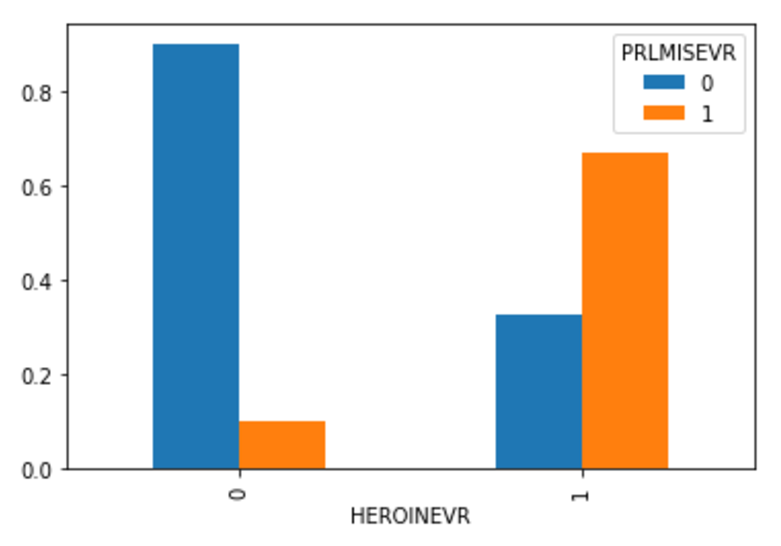
\includegraphics[width=\columnwidth]{images/Figure1.pdf}
  \caption{Proportion of Individuals Who Reported Ever Misusing Prescription
  Opioid Pain Relievers and Proportion Who Reported Using Heroin}
  \label{f:Figure1}
\end{figure}

%%%%%%%%%%%%%%%%%%%%%%%%%%%%%%%%%%%%%%%%%%%%%%%%%%%%%%%%%%%%%%%%%%%%%%%%%%%%%%%%

Figure 2 shows the aggregated measure of Opioid Pain Reliever misuse and abuse 
plotted against the aggregated measure of Heroin use (which includes misuse, 
abuse, lifetime use, past year use, 30 day use), with weighted regression 
lines grouped by size of City Metropolitan region (from none to large). 
The largest proportion of the sample who report prescription opioid misuse, 
abuse, and heroin use is represented by observations from large metropolitan 
areas (red circles) with large population size. However, a small number of
observations from rural or small metropolitan regions (blue and green circles)
showed very high rates of prescription opioid misuse and abuse. Regression 
lines (i.e., line of best fit) shown are weighted by the City/Metro
region attribute, with a steeper slope shown for smaller metropolitan regions 
than large metropolitan regions. The difference in slope may be due to the 
influence of the small number of outliers who had high degrees of prescription 
opioid misuse, and heroin use. The plot also shows a clear divide on the y-axis,
which separates the sample according to high and low or no prescription opioid 
misuse, although the continuum of heroin use from no, low, to high is 
distributed fairly evenly along the x-axis. 


\begin{figure}[!ht]
  \centering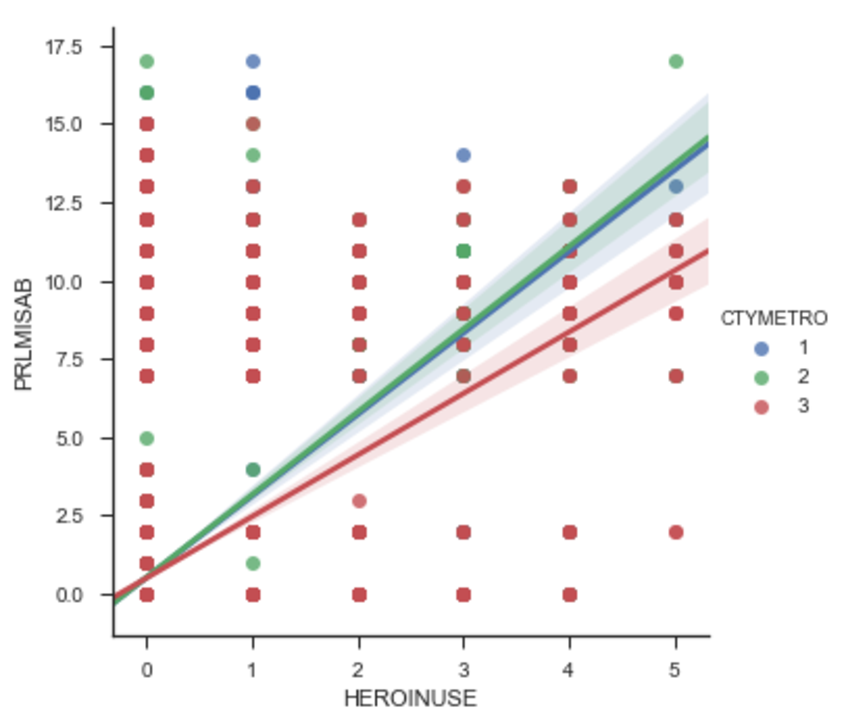
\includegraphics[width=\columnwidth]{images/Figure2.pdf}
  \caption{Plot of Opioid Pain Medication Misuse and Abuse and Heroin Use
  with Regression Slopes Weighted by Metropolitan Area Size}
  \label{f:Figure2}
\end{figure}

%%%%%%%%%%%%%%%%%%%%%%%%%%%%%%%%%%%%%%%%%%%%%%%%%%%%%%%%%%%%%%%%%%%%%%%%%%%%%%%%

Figure 3 shows the pairplots of demographic features including mental health
(higher scores equal to more depression), 

\begin{figure}[!ht]
  \centering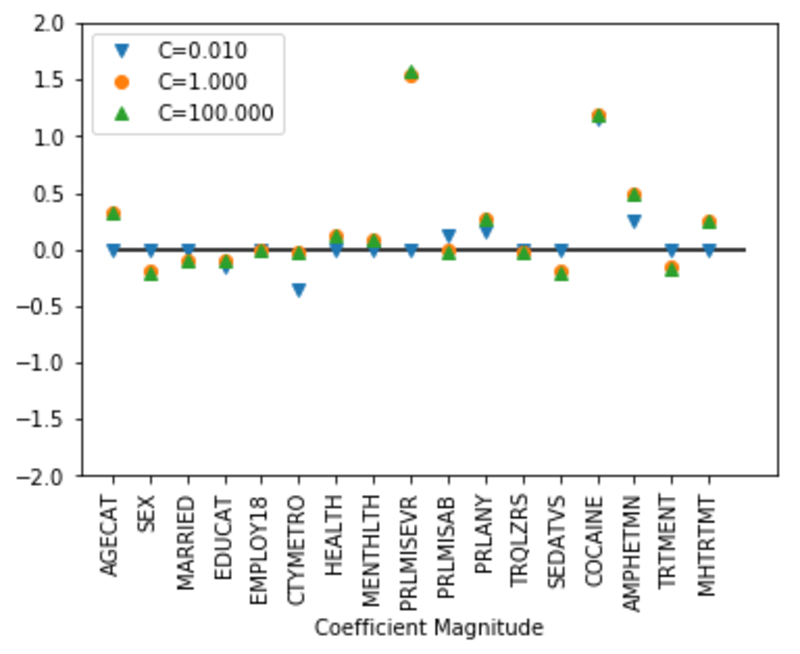
\includegraphics[width=\columnwidth]{images/Figure3.pdf}
  \caption{Pairplots of Mental Health, Prescription Opioid Misuse and Abuse,
  Heroin Use, and Size of City Metropolitan Area}
  \label{f:Figure3}
\end{figure}


%%%%%%%%%%%%%%%%%%%%%%%%%%%%%%%%%%%%%%%%%%%%%%%%%%%%%%%%%%%%%%%%%%%%%%%%%%%%%%%%
\subsection{Classifier Models of Heroin Use}

This analysis classified individuals according to whether they had ever used 
heroin (i.e., ``Heroin Use Ever``. All classifier models were constructed using 
SciKit Learn \cite{muller17} using an interactive python jupyter notebooks  
\cite{classifyH}. In addition to identifying the accuracy of the model, 
classification can identify features in terms of importance for classifying the 
outcome. The features of interest were identified: demographic characteristics, 
health, mental health (adultdepression), prescription opioid misuse and abuse 
('PRLMISEVR', 'PRLMISAB', 'PRLANY'), prescription tranquilizers and sedatives 
('TRQLZRS', 'SEDATVS'), illicit drugs ('COCAINE', 'AMPHETMN'), drug treatment 
('TRTMENT'), and mental health treatment ('MHTRTMT'). The target variable was 
heroin use ('HEROINEVR'). Next, the dataset was split into the training set 
and test sets using the `train-test-split` function in `sklearn`.

%%%%%%%%%%%%%%%%%%%%%%%%%%%%%%%%%%%%%%%%%%%%%%%%%%%%%%%%%%%%%%%%%%%%%%%%%%%%%%%%
\subsubsection{Logistic Regression Classifier}

Logistic Regression Classification is a based on a linear equation that 
calculates the relative weight of each feature for a categorical target or 
binary outcome (``yes/no``). The logistic regression classifier was fit to 
the training data, and the model was validated on the test data. By default, 
the model applies L2 (Ridge) regularization, and the test set accuracy 
was 0.983 and test set accuracy was 0.984. Parameter `C` determines the 
strength of regularization; higher values of C provides greater regularization. 
The L1 (Lasso) regularization limits the values of most coefficients to zero, 
creating a more interpretable model using only a few features. Figure 4 plots 
the Coefficients of Logistic Regression Classifier (LGC) for Heroin Use with 
L1 (Lasso) regularization under different values of parameter C. The default 
setting, C=1.0, provides good performance for train and test sets, but the 
model is very likely underfitting the test data. Using a higher value of C 
fits a more 'flexible' model and generally gives improved accuracy for both 
training and tests sets. A value of C=100 yielded training set accuracy of
0.98 and test set accuracy of 0.98. Figure 4 shows that Pain Reliever Misuse
('PRLMISEVR'), Cocaine use, and Amphetamine use, were the three features
with the highest coefficient values for classifying Heroin use. 

\begin{figure}[!ht]
  \centering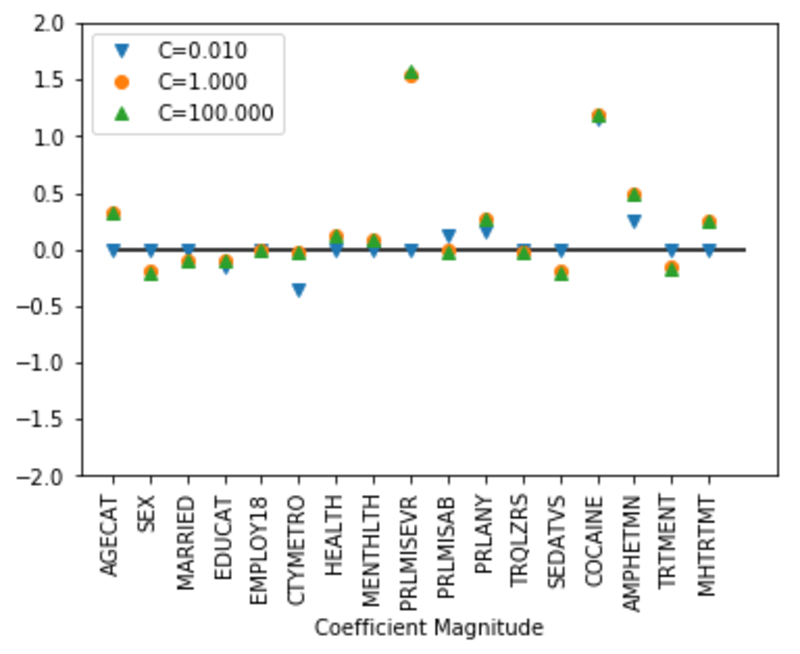
\includegraphics[width=\columnwidth]{images/Figure4.pdf}
  \caption{Coefficients of Logistic Regression Classifier of Heroin Use 
  (With L1 Penalty and Values of Regularization Parameter C)}
  \label{f:Figure4}
\end{figure}

\cite{raschka17}

%%%%%%%%%%%%%%%%%%%%%%%%%%%%%%%%%%%%%%%%%%%%%%%%%%%%%%%%%%%%%%%%%%%%%%%%%%%%%%%%
\subsubsection{Decision Tree Classifier}

Decision Trees Classification of Heroin Use was implemented using the `Decision 
Tree Classifier` package in scikit-learn, which only does pre-pruning. First, 
the decision model was build using the default setting of a fully developed 
tree until all leaves are pure. The `random state` features is fixed to break 
ties internally. 

Without restricting their depth, decision trees can become complex; unpruned 
trees are prone to overfitting and do not generalize well to new data. 

A second analysis applies pre-pruning, by setting the maximum depth to 4, which
means the algorithm will split on the four consecutive questions. Limiting
the depth of the tree decreases overfitting, which results in lower accuracy
on the training set, but imporoved performance on the test set. 

Even with a  tree depth of 4, the tree can be a bit complex. Figure 5 shows a 
partial view of the resulting decision tree classifier of heroin use because 
the complete figure was too wide to include here.

Instead of looking at the whole tree, features importance is a commonly used 
summary function that rates how important each feature is for the decisions 
which a tree makes. Each feature is assigned an importance value between 0 and 1;
with a value of 1 indicating that the feature perfectly predicts the target and 
a value of 0 that the feature was not used at all. Feature importance values
always sum to 1. A feature may be assigned a low feature importance value
because another feature encodes the same information \cite{muller17}.



\begin{figure}[!ht]
  \centering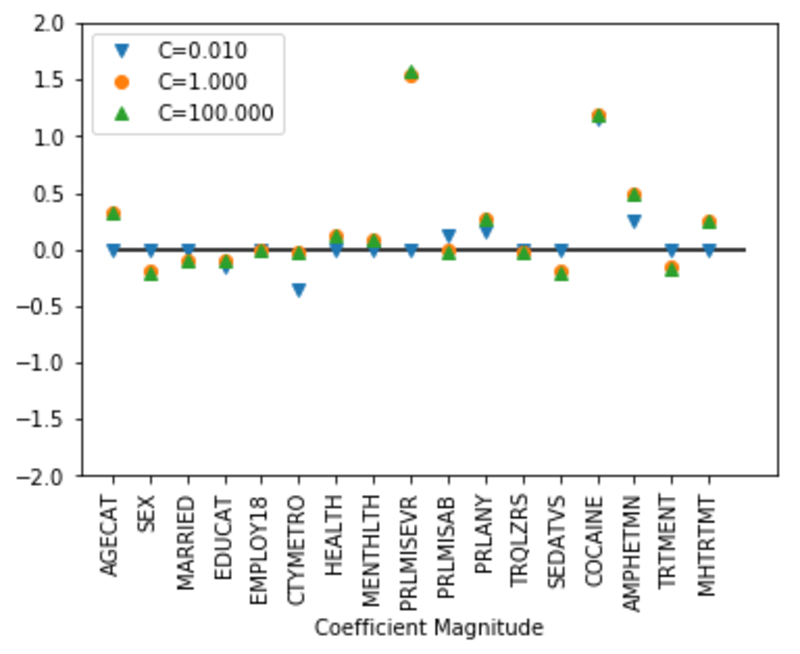
\includegraphics[width=\columnwidth]{images/Figure5.pdf}
  \caption{Decision Tree Classification of Heroin Use (Partial View)}
  \label{f:Figure5}
\end{figure}

\begin{figure}[!ht]
  \centering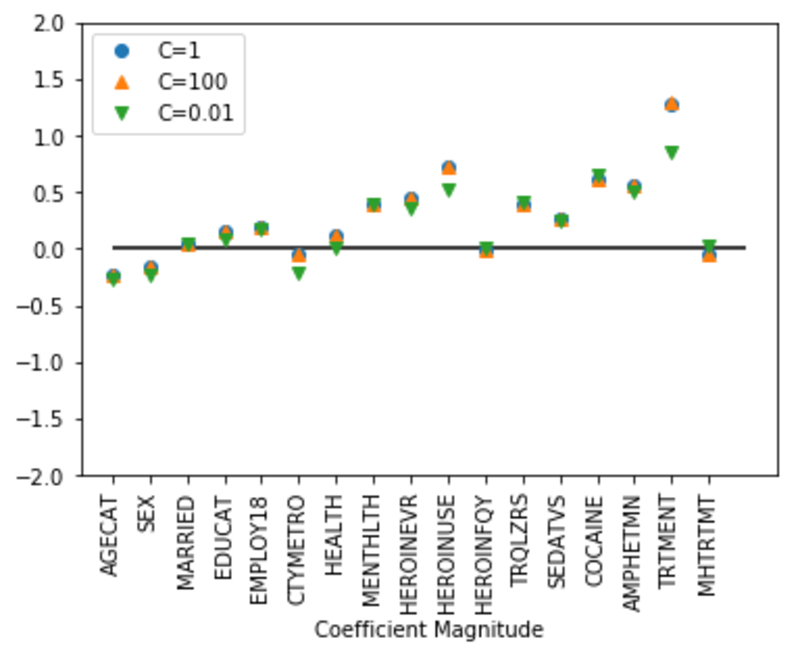
\includegraphics[width=\columnwidth]{images/Figure6.pdf}
  \caption{Feature Importance for Decision Tree Classifier for Heroin Use}
  \label{f:Figure9}
\end{figure}

%%%%%%%%%%%%%%%%%%%%%%%%%%%%%%%%%%%%%%%%%%%%%%%%%%%%%%%%%%%%%%%%%%%%%%%%%%%%%%%%
\subsubsection{Random Forests Classifier}

Random forests is an ensemble approach that builds many trees and averages 
their results to reduce overfitting. The random forest classifier function was 
used in sklearn, and the parameters of interest were the (1) the number of 
trees to build (i.e., n-estimators), (2) the number of data points selected
in our bootstrap sampling (i.e., n-samples), and (3) the maximum number of 
features considered at each decision node branch (i.e., max-features). The
max-features parameter determines how random each tree is, with smaller 
values of max-features resulting in trees in the random forest that are very 
different from each other. 

Feature importance for random forests is computed by aggregating the feature 
importance over trees in the random forest, and typically provides a more 
reliable measure than feature importance for a single tree. 

\begin{figure}[!ht]
  \centering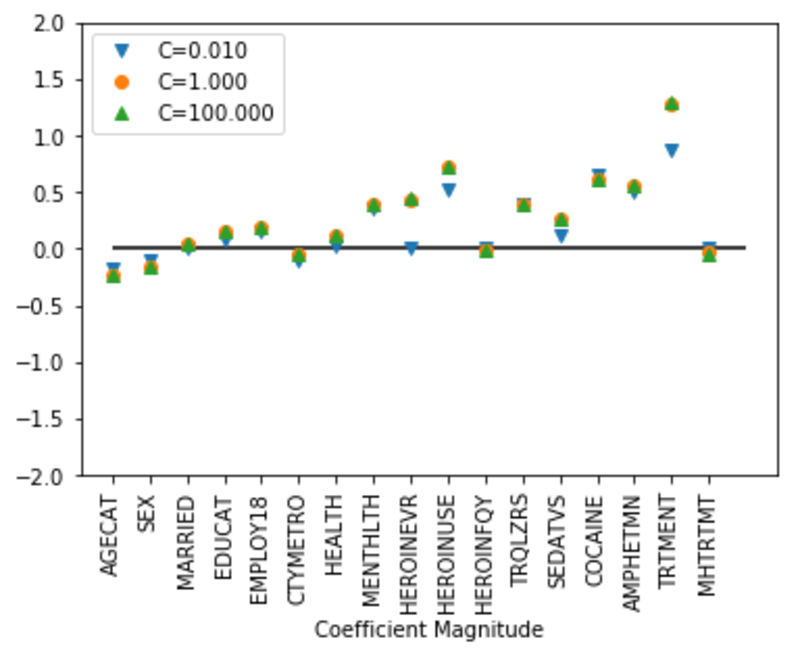
\includegraphics[width=\columnwidth]{images/Figure7.pdf}
  \caption{Feature Importance for Random Forests Classifier for Heroin Use}
  \label{f:Figure7}
\end{figure}

%%%%%%%%%%%%%%%%%%%%%%%%%%%%%%%%%%%%%%%%%%%%%%%%%%%%%%%%%%%%%%%%%%%%%%%%%%%%%%%%
\subsubsection{Gradient Boosting Classifier}


\begin{figure}[!ht]
  \centering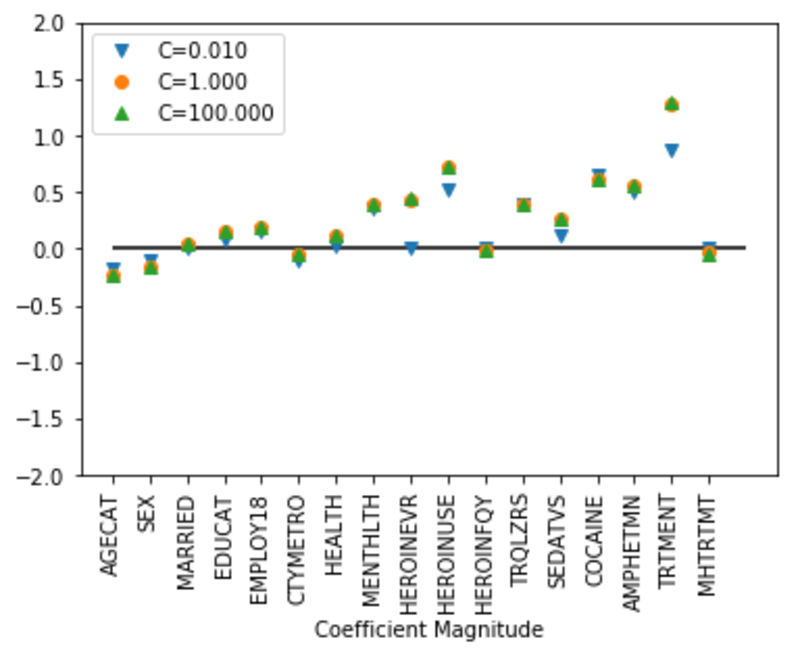
\includegraphics[width=\columnwidth]{images/Figure8.pdf}
  \caption{Feature Importance for Gradient Boosting Classifier for Heroin Use}
  \label{f:Figure8}
\end{figure}



%%%%%%%%%%%%%%%%%%%%%%%%%%%%%%%%%%%%%%%%%%%%%%%%%%%%%%%%%%%%%%%%%%%%%%%%%%%%%%%%
\subsection{Classifier Models of Prescription Opioid Pain Relievers Misuse}

\subsubsection{Logistic Regression Classifier}


\cite{classifyPRL}

\begin{figure}[!ht]
  \centering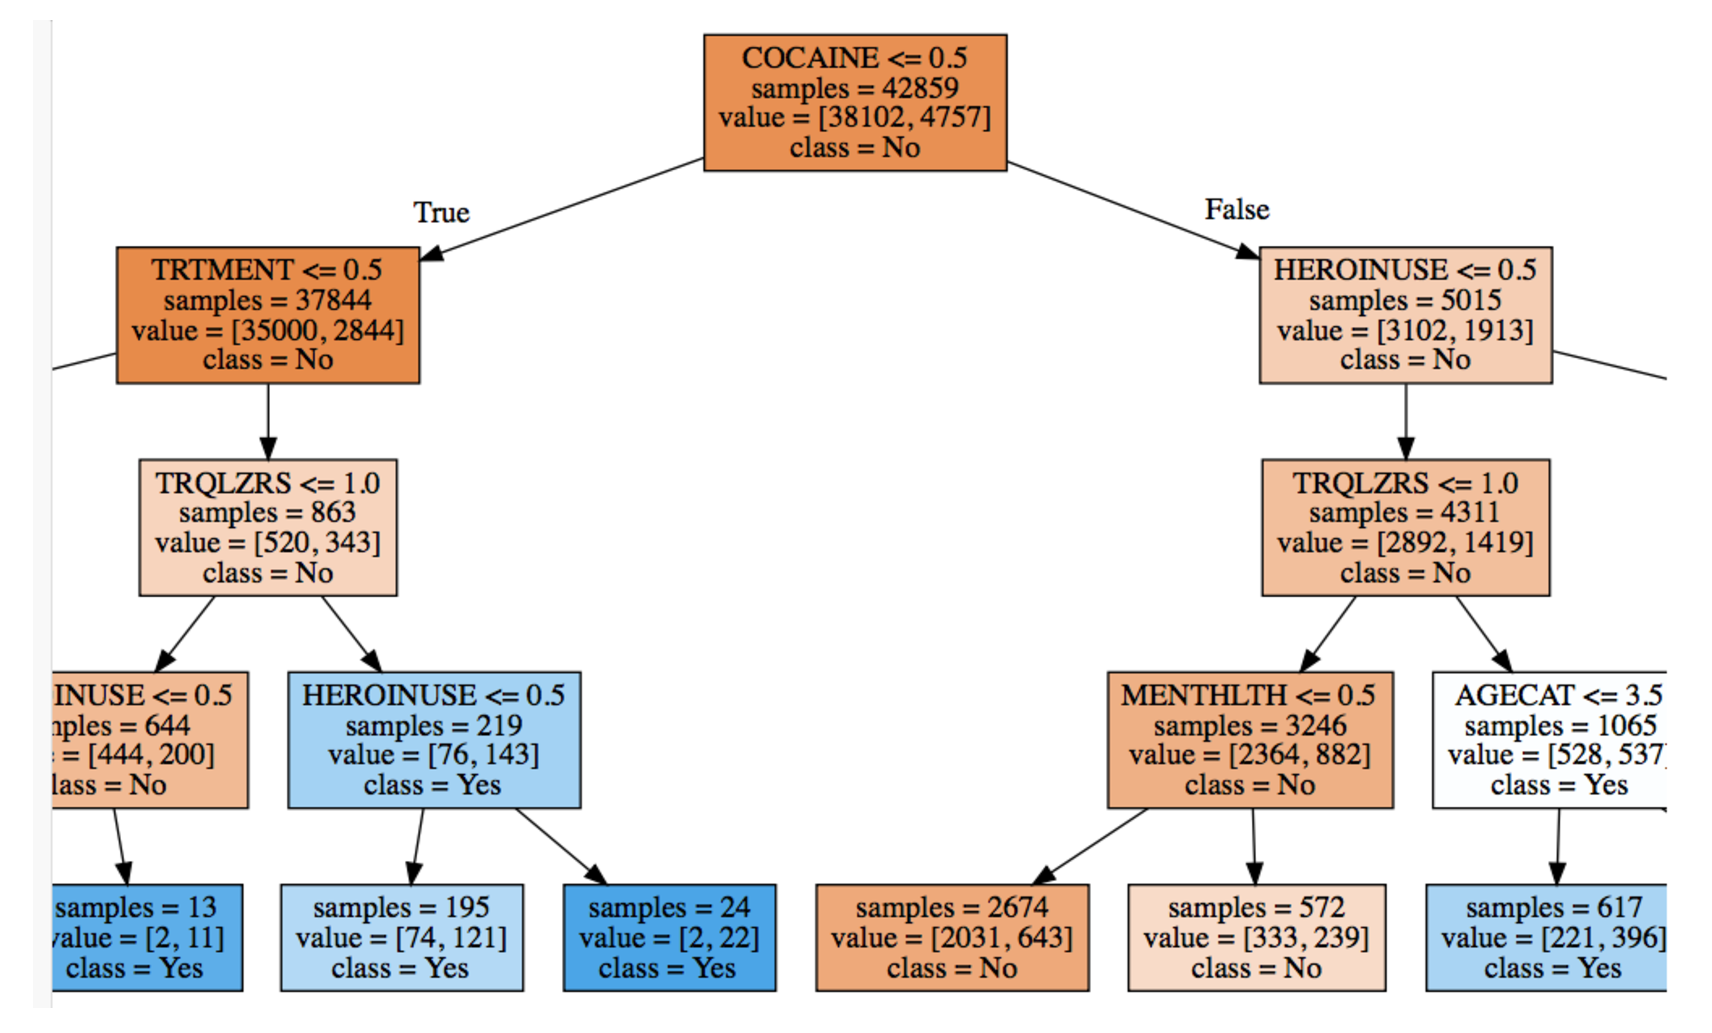
\includegraphics[width=\columnwidth]{images/Figure9.pdf}
  \caption{Logistic Regression Classification of Opioid Pain Medication
  with L2 Lasso Regularization}
  \label{f:Figure9}
\end{figure}

\cite{vanderplas17}

\subsubsection{Decision Tree Classifier\cite{muller17}}

%%%%%%%%%%%%%%%%%%%%%%%%%%%%%%%%%%%%%%%%%%%%%%%%%%%%%%%%%%%%%%%%%%%%%%%%%%%%%%%%
\section{Discussion}

\subsection{Extension to Big Data}

The methods used in this project could be extended to better approximate 
big data for health analytics in the following ways: (1) Include a larger 
selection of features from the 2600 attributes in in the NSDUH-2015 dataset; 
(2) Include survey data from previous years (e.g., 2005-2015); and (3) 
Extend the sample to the population of patients who have been prescribed 
opioid pain medication. There were many additional features that could have
been included in the subset of features included in the project dataset. 
However, data cleaning and preparation can be a time consuming process, 
especially for datasets with a large number of features \cite{rahm00}. 
Additional data from the NSDUH was downloaded from previous years (2012 to 
2014), and a preliminary examination of the data revealed inconsistencies 
in questions and prescription opioid medications that would need to be 
resolved in order to combine data from multiple years. In addition to data 
cleaning, there are several steps involved in the consolidation of data from 
multiple sources into a single dataset, which include extraction, integration, 
and aggregation of features. Unfortunately, time constraints for the project 
deadline did not allow for the inclusion of data from previous years into this 
analysis. A future study could integrate data from different years into the
analysis or include data from multiple sources. 


%%%%%%%%%%%%%%%%%%%%%%%%%%%%%%%%%%%%%%%%%%%%%%%%%%%%%%%%%%%%%%%%%%%%%%%%%%%%%%%%
\subsection{Limitations}

To be of any use, diverse and often messy raw data has to be sifted through and 
effectively organized for further analysis, and 

there are legitimate questions about the reliability of self report data from 
surveyresearch for predicting actual behavior. 

The question of Value evaluates the quality of the data as it pertains to 
intended outcomes, such as limiting the spread of contagion and disease 
prevention. 

An important challenge for making sense of big data is developing analytic 
tools adequate to handle large volumes of data in real time.

%%%%%%%%%%%%%%%%%%%%%%%%%%%%%%%%%%%%%%%%%%%%%%%%%%%%%%%%%%%%%%%%%%%%%%%%%%%%%%%%
\subsection{Drug Abuse, Dependency, and Addiction}

Drug addiction has many similar characteristics to other chronic medical 
illnesses, but there are unique challenges to the treatment of addiction
\cite{marsch12, swendson16}. In drug rehabilitation treatment programs, 
patients undergo intense detoxification that reduces their drug tolerance, but 
are then released back into the environments associated with their drug use, 
putting them at high risk for relapse and potential drug overdose 
\cite{johnson11}. According to a classical conditioning model of addiction, 
situational cues or events can elicit a motivational state underlying relapse 
to drug use. Addictive behavior can be also be reinstated after extinction of 
dependency by exposure to drug-related cues or stressors in the environment 
\cite{shaham03}. 


%%%%%%%%%%%%%%%%%%%%%%%%%%%%%%%%%%%%%%%%%%%%%%%%%%%%%%%%%%%%%%%%%%%%%%%%%%%%%%%%
\subsection{Dynamics of Epidemic Spreading}

As described in the introduction, prescription opioid addiction and overdose 
death is a major health crisis that has been described as an epidemic.
The expansion of pioid addiction may thought of as analogous to examples of
biological epidemics in that spreading proceeds as a dynamic process based on 
interactions between infected and uninfected persons. The dynamics of 
epidemic spreading is complex, involving networks of person-to-person contact, 
indirect contact exposure, and transportation pathways such as roads and 
highways and airline transportation network \cite{Colizza06}, that facilitate 
the distribution of opioid drugs to individuals susceptible to addiction and 
dependency. This project has identified some of the features important for 
classifying heroin use and prescription opioid misuse. 

Epidemics are quantified in terms of the proportion of the population infected, 
those yet to be infected, and the rate of transmission, and the structure of the 
contact network can influence epidemic spreading \cite{pastor01}. 

For example, in the case of simple contagion, weak ties among 
acquaintances or infrequent associations provide shortcuts between distant nodes 
that reduce distance within the network \cite{granovetter73} and can facilitate 
the spread of disease. 

Furthermore, networks with ``small world'' properties have many nodes with 
few connections, but a small number of highly connected nodes that can rapidly 
transmit contagion throughout the network \cite{watts98}. Analyzing the 
correlation between Twitter posts and rate of ILI reports does not capture the 
complex network structure that underlies disease epidemics and pandemics. 
It is possible that by analyzing the structure of social media networks, 

Could use network analysis to examine opioid distribution pathways and points 
of contact among nodes or person in the network of prescription medications.
The opioid crisis in North America may be amenable to social network modeling as 
drug usage, dependancy, and addiction is subserved by social networks. 

future research may help to identify how points of connection within online
networks are associated with the spread of contagion and resulting epidemics 
\cite{zhu17}. 


%%%%%%%%%%%%%%%%%%%%%%%%%%%%%%%%%%%%%%%%%%%%%%%%%%%%%%%%%%%%%%%%%%%%%%%%%%%%%%%%
\section{Conclusion}

Several machine learning methods were used to classify heroin use and 
prescription opioid misuse and abuse. The results of this analysis are somewhat inconclusive, given that the direction of these effect is unknown. On the one 
hand there is evidence that individual who reported having used heroin were 
also more likely to report misusing or abusing prescription opioids. On the 
other hand, the proportion of individuals who misused or abused prescription 
opioids, and also reported using heroin, was twice as large as the proportion 
who reported only using heroin. A general conclusion is that the results 
provide partial support for the hypothesis that taking prescription opioids
leads to a higher likelihood of illicid opioid use. However, the results did
not provide sufficienbt evidence to rule out the alternative hypothesis that
people who have used heroin may have a propensity for opioid use therefore
be more likely to become dependent on prescription opioid medications. Given
that the number of individuals who reported using heroin in this sample was
low, additional data may help to provide evidence to resolve this question.
A limitation of survey data is there may be bias in self-reports of illicit
drug use, as it is a proscribed and illegal behavior, and therefore the 
data may underestimate the actual rate of heroin use in the general population. 
Including additional data from previous years may provide a more tests of 
these hypotheses. 


Machine of opioid abuse can contribute to efforts to 
address prescription opioid addiction, overdoses, in the following ways: 
\begin{enumerate}
\item Identify factors related to opioid dependency
\item Inform consumers of opioid medication as to risk factors 
\item Increase knowledge of opioid abuse for more informed prescriptions. 
\end{enumerate}



%%%%%%%%%%%%%%%%%%%%%%%%%%%%%%%%%%%%%%%%%%%%%%%%%%%%%%%%%%%%%%%%%%%%%%%%%%%%%%%%
\begin{acks}

The author would like to thank Dr. Gregor von Laszewski, the Teaching 
Assistants, Juliette Zurick, Miao Jiang, Hungri Lee, Grace Li, Saber Sheybani
Moghadam, and others who helped to improve this project and report.

\end{acks}

\bibliographystyle{ACM-Reference-Format}
\bibliography{report} 


%%%%%%%%%%%%%%%%%%%%%%%%%%%%%%%%%%%%%%%%%%%%%%%%%%%%%%%%%%%%%%%%%%%%%%%%%%%%%%%%
\appendix

\section{Code References}
All code, notebooks, files, and folders for this project can be found in the
i523/hid335/project githup repository: 
\url{url:  https://github.com/bigdata-i523/hid335/tree/master/project}.

\subsection{Download and Extract Data file}

The `get-data.py` function was written to download the data, unzip the data
files, extract the data, and write the NSDUH-2015 dataset to CSV file 
\cite{getdata17}.

%%%%%%%%%%%%%%%%%%%%%%%%%%%%%%%%%%%%%%%%%%%%%%%%%%%%%%%%%%%%%%%%%%%%%%%%%%%%%%%%
\subsection{Data Cleaning and Preparation}

Data cleaning and preparation steps was conducted using an interactive python Jupyter Notebook \cite{data17} based on examples in Python for Data Analysis \cite{mckinney17} and the Python Data Science Handbook \cite{vanderplas17}.

\subsection{Exploratory Data Analysis}

Exploratory Data Analysis and Visualization was conducted using an interactive
python notebook: CITE URL

based on examples from Python for Data Analysis \cite{mckinney17}, and the 
Python Data Science Handbook \cite{vanderplas17}.  

%%%%%%%%%%%%%%%%%%%%%%%%%%%%%%%%%%%%%%%%%%%%%%%%%%%%%%%%%%%%%%%%%%%%%%%%%%%%%%%%
\subsection{Machine Learning Classifier Algorithms}
Machine learning classification models included logistic regression classifier, 
decision Tree classifier, random forests classifier, and gradient boosting 
classifier were constructed using SciKit Learn \cite{muller17, raschka17} 
using two separate interactive python jupyter notebook, one for classifying 
Heroin Use as the target variable \cite{classifyH}, and another notebook for classifying Prescription Opioid Misuse as the target \cite{classifyPRL}. 


%\begin{enumerate}

%\item Do not to use the underscore in bibtex labels
%\item Address each of the items in the issues.tex file  
%item Please do this only at the end once you have finished writing the paper. 
%\item Change `TODO` with `DONE`. 

%\end{enumerate}

%\section{Issues}

\DONE{Example of done item: Once you fix an item, change TODO to DONE}

\subsection{Assignment Submission Issues}

    \DONE{Do not make changes to your paper during grading, when your repository should be frozen.}

\subsection{Uncaught Bibliography Errors}

    \DONE{Missing bibliography file generated by JabRef}
    \DONE{Bibtex labels cannot have any spaces, \_ or \& in it}
    \DONE{Citations in text showing as [?]: this means either your report.bib is not up-to-date or there is a spelling error in the label of the item you want to cite, either in report.bib or in report.tex}

\subsection{Formatting}

    \DONE{Incorrect number of keywords or HID and i523 not included in the keywords}
    \DONE{Other formatting issues}

\subsection{Writing Errors}

    \DONE{Errors in title, e.g. capitalization}
    \DONE{Spelling errors}
    \DONE{Are you using {\em a} and {\em the} properly?}
    \DONE{Do not use phrases such as {\em shown in the Figure below}. Instead, use {\em as shown in Figure 3}, when referring to the 3rd figure}
    \DONE{Do not use the word {\em I} instead use {\em we} even if you are the sole author}
    \DONE{Do not use the phrase {\em In this paper/report we show} instead use {\em We show}. It is not important if this is a paper or a report and does not need to be mentioned}
    \DONE{If you want to say {\em and} do not use {\em \&} but use the word {\em and}}
    \DONE{Use a space after . , : }
    \DONE{When using a section command, the section title is not written in all-caps as format does this for you}\begin{verbatim}\section{Introduction} and NOT \section{INTRODUCTION} \end{verbatim}

\subsection{Citation Issues and Plagiarism}

    \DONE{It is your responsibility to make sure no plagiarism occurs. The instructions and resources were given in the class}
    \DONE{Claims made without citations provided}
    \DONE{Need to paraphrase long quotations (whole sentences or longer)}
    \DONE{Need to quote directly cited material}

\subsection{Character Errors}

    \DONE{Erroneous use of quotation marks, i.e. use ``quotes'' , instead of " "}
    \DONE{To emphasize a word, use {\em emphasize} and not ``quote''}
    \DONE{When using the characters \& \# \% \_  put a backslash before them so that they show up correctly}
    \DONE{Pasting and copying from the Web often results in non-ASCII characters to be used in your text, please remove them and replace accordingly. This is the case for quotes, dashes and all the other special characters.}
    \DONE{If you see a figure and not a figure in text you copied from a text that has the fi combined as a single character}

\subsection{Structural Issues}

    \DONE{Acknowledgement section missing}
    \DONE{Incorrect README file}
    \DONE{In case of a class and if you do a multi-author paper, you need to add an appendix describing who did what in the paper}
    \DONE{The paper has less than 2 pages of text, i.e. excluding images, tables and figures}
    \DONE{The paper has more than 6 pages of text, i.e. excluding images, tables and figures}
    \DONE{Do not artificially inflate your paper if you are below the page limit}

\subsection{Details about the Figures and Tables}

    \DONE{Capitalization errors in referring to captions, e.g. Figure 1, Table 2}
    \DONE{Do use {\em label} and {\em ref} to automatically create figure numbers}
    \DONE{Wrong placement of figure caption. They should be on the bottom of the figure}
    \DONE{Wrong placement of table caption. They should be on the top of the table}
    \DONE{Images submitted incorrectly. They should be in native format, e.g. .graffle, .pptx, .png, .jpg}
    \DONE{Do not submit eps images. Instead, convert them to PDF}

    \DONE{The image files must be in a single directory named "images"}
    \DONE{In case there is a powerpoint in the submission, the image must be exported as PDF}
    \DONE{Make the figures large enough so we can read the details. If needed make the figure over two columns}
    \DONE{Do not worry about the figure placement if they are at a different location than you think. Figures are allowed to float. For this class, you should place all figures at the end of the report.}
    \DONE{In case you copied a figure from another paper you need to ask for copyright permission. In case of a class paper, you must include a reference to the original in the caption}
    \DONE{Remove any figure that is not referred to explicitly in the text (As shown in Figure ..)}
    \DONE{Do not use textwidth as a parameter for includegraphics}
    \DONE{Figures should be reasonably sized and often you just need to
  add columnwidth} e.g. \begin{verbatim}/includegraphics[width=\columnwidth]{images/myimage.pdf}\end{verbatim}

re


\end{document}
